\documentclass[12pt]{article}

\usepackage[margin=1in]{geometry}
\usepackage{amsmath,amsthm,amssymb}
\usepackage{bbold}
\usepackage{braket}
\usepackage{mathtools}

\newcommand{\Tr}[1]{\text{Tr}[#1]}
\renewcommand{\exp}[1]{e^{#1}}

\newcommand{\aside}[2]{#1}
\newcommand{\link}[2]{#1}
\newcommand{\todo}[1]{(#1)}

\begin{document}

\title{Poincare Group and the Definition of a Particle}
\author{}
\date{}

\maketitle

\section{Introduction}
The Poincare group is a combination of the translation group, which consists of translations in the 4 dimensions of spacetime, and the Lorentz group, which consists of boosts, rotations, parity, and time reversal. It is of particular interest to us because \aside{every relativistic theory we come up with must be Poincare invariant}{Ignoring general relativity, in which Poincare invariance is only local.}.

The primary result of this chapter is to give a mathematical definition for a particle. We will associate particles with irreducible representations of the Poincare group, and this will automatically give our particles mass and spin. The components of spin for a particle will depend on if the particle is massless or massive. We will see that massive particles can have spin components in 3 directions, like we are used to with $\hat{J}_i$ for $i=1,2,3$. However, massless particles can only have spin in the direction of its momentum, and we will call that property helicity.

Now that you have an idea of where we are heading, we need to pan out our journey. First, we will need to look closely at the generators of the group and classify its irreducible representations. Then we will discuss something called the Pauli-Lubanski pseudovector, which will give rise to spin. Then we will talk about how to define a particle. Lastly, we will look at particles with mass and particles without mass and see the properties of both.

\section{Generators}
Our first main goal is to classify the irreducible representations of the Poincare group. We would like to find a nice basis for the vector space these representations act on that are labelled by eigenvalues of some of the generators of the group. In order to do that, we need to know the commutation relations between the generators so that we can figure out which generators can be simultaneously diagononalized.

Translations in spacetime has 4 degrees of freedom: 1 for time translations and 3 for spatial translations. So, we need 4 generators. We can neatly store 4 components into a 4-vector, so let's call them $P^\mu$. Next, Lorentz transformations have 6 degrees of freedom: 3 for rotations and 3 for boosts. To still use our 4-vector notation, we say that the generators are $M^{\mu\nu}$ with the constraint that $M^{\mu\nu}=-M^{\nu\mu}$, i.e. they are antisymmetric under $\mu\leftrightarrow\nu$.
\begin{equation}
    \text{Poincare Group Generators: } P^\mu, M^{\mu\nu}=-M^{\nu\mu}
\end{equation}

I want to stress that all we have assumed here is the number of generators. $P^\mu$ certaintly looks like it is the momentum, but we don't know that (yet). All we know is there are 4 generators and we have this already existing slick 4-vector notation that neatly groups 4 objects together.

Additionally, requiring $M^{\mu\nu}$ to be antisymmetric under exchange of indices is again only a nice use of notation to get only 6 generators. We could have chosen a notation of something else, say $M_i$ for $i=1\dots6$, but that doesn't really match with any existing physics notation that is used often.

One last comment before we move one: $M^{\mu\nu}$ refers to an entire matrix, not a specific component of a matrix. It is the 6 generators that are labelled by $\mu$ and $\nu$. If we wanted to reference a specific element, we would need to say $(M^{\mu\nu})_{\alpha\beta}$. Having multiple sets of indices that refer to different classes of objects will be a common theme throughout quantum field theory.

Now that we know what the generators are, we want to know what their commutation relations are.
\begin{equation}
    [P^\mu,P^\nu]=\text{?}\qquad[M^{\mu\nu},P^\sigma]=\text{?}\qquad[M^{\mu\nu},M^{\rho\sigma}]=\text{?}
\end{equation}

We will find these by using group multiplication and representations. As you know, a representation must be faithful to the group multiplication rule. For group elements $g_1$ and $g_1$ and representation $D$,
\begin{equation}
    D(g_1)D(g_2)=D(g_1g_2)
\end{equation}

Thus, we need to find what the group multiplication rule for the Poincare group is. We will label a specific Poincare group member by the pair $(\Lambda,a)$, where $\Lambda$ is the Lorentz transformation matrix and $a$ is the translation vector (with indices suppressed). We know how this acts on a coordinate $x^\mu$:
\begin{equation}
    x^\mu\rightarrow{\Lambda^\mu}_\nu x^\nu+a^\mu
\end{equation}

Now consider when we act on $x^\mu$ with two successive Poincare transformations $(\Lambda_1,a_1)$ and $(\Lambda_2,a_2)$.
\begin{equation}
    x^\mu\xrightarrow{1}{\Lambda_1^\mu}_\nu x^\nu+a_1^\mu\xrightarrow{2} {\Lambda_2^\mu}_\nu{\Lambda_1^\nu}_\alpha x^\alpha+{\Lambda_2^\mu}_\nu a_1^\nu +a_2^\mu
\end{equation}

We can read off now the combination of two Poincare transformations.
\begin{equation}
    (\Lambda_2,a_2)(\Lambda_1,a_1)\rightarrow(\Lambda_2\Lambda_1,\Lambda_2 a_1 + a_2)
\end{equation}

So, any representation of the Poincare group must be faithful to this. From now on we will talk in terms of representations $D(\Lambda,a)$ instead of the pair $(\Lambda,a)$.
\begin{equation}
    D(\Lambda_2,a_2)D(\Lambda_1,a_1)\rightarrow D(\Lambda_2\Lambda_1,\Lambda_2 a_1 + a_2)
\end{equation}

One consequence of this multiplication rule is that a Poincare transformation can be split into a pure translation and pure Lorentz transformation.
\begin{equation}
    D(\Lambda,a)=D(\mathbb{1},a)D(\Lambda,0)
\end{equation}

Note that this doesn't work the other way around.
\begin{equation}
    D(\Lambda,0)D(\mathbb{1},a)=D(\Lambda,\Lambda a)\neq D(\Lambda,a)
\end{equation}

We already know the generators of translations and Lorentz transformations, so we can write down the representations for each.
\begin{equation}
    D(\mathbb{1},a)=e^{i a_\mu P^\mu}
\end{equation}
\begin{equation}
    D(\Lambda,p)=e^{\frac{i}{2}\omega_{\mu\nu}M^{\mu\nu}}
\end{equation}

We have preemptively added a factor of $\frac{1}{2}$ to the Lorentz group transformation because $\omega_{\mu\nu}$ is antisymmetric (which we will now show), so $\omega_{\mu\nu}M^{\mu\nu}$ is symmetric under exchange of $\mu$ and $\nu$. Thus, we divide by $2$ to avoid overcounting. 

To show that $\omega_{\mu\nu}$ is antisymmetric, we need to remember that Lorentz transformations are defined by $\Lambda^T g \Lambda =g$ for the metric tensor $g$. Putting these into index notation, we can get rid of the metrics tensors.
\begin{equation}
    \Lambda^Tg\Lambda=g\rightarrow{(\Lambda^T)^\alpha}_\mu g^{\mu\nu} {\Lambda_\nu}^\beta={\Lambda_\mu}^\alpha g^{\mu\nu} {\Lambda_\nu}^\beta=\Lambda^{\nu\alpha}{\Lambda_\nu}^\beta\rightarrow{\Lambda_\nu}^\alpha{\Lambda^\nu}_\beta={\delta^\alpha}_\beta
\end{equation}

If take take an infinitesimal Lorentz transformation ${\Lambda^\mu}_\nu={\delta^\mu}_\nu+{\omega^\mu}_\nu+\cdots$, we can plug these in and look at everything to first order.
\begin{equation}
    ({\delta_\nu}^\alpha+{\omega_\nu}^\alpha)({\delta^\nu}_\beta+{\omega^\nu}_\beta)={\delta^\alpha}_\beta+{\omega_\beta}^\alpha +{\omega^\alpha}_\beta+O(\omega^2)
\end{equation}

This is all equal to ${\delta^\alpha}_\beta$, which cancels on both sides. Thus, looking at the first order terms, we can say that $\omega_{\mu\nu}=-\omega_{\nu\mu}$.

Now, equipped with the group multiplication rule and representation for both translations and Lorentz transformation, we can derive the commutation relations. These will be done in full detail in the appendices because they can get quite lengthy. In short, we will look at the representation of different multiplications to arrive at our commutation relations. Below show which multiplications give rise to which commutation relations.
\begin{equation}
\begin{alignedat}{2}
    D(\mathbb{1},a_1)D(\mathbb{1},a_2)&=D(\mathbb{1},a_1+a_2)\quad &&\rightarrow \quad [P^\mu,P^\nu] \\
    D(\Lambda,0)D(\mathbb{1},a)&=D(\Lambda,\Lambda a) &&\rightarrow \quad [M^{\mu\nu},P^\sigma] \\
    D(\Lambda_1,0)D(\Lambda_2,0)&=D(\Lambda_1\Lambda_2,0) &&\rightarrow \quad [M^{\mu\nu},M^{\rho\sigma}]
\end{alignedat}
\end{equation}

Without further ado, we present the commutation relations between the generators of the Poincare group.
\begin{equation}
\begin{aligned}
    [P^\mu,P^\nu]&=0 \\
    [M^{\mu\nu},P^\sigma] &= i(P^\nu g^{\mu\sigma}-P^\mu g_{\nu\sigma})\\
    [M^{\mu\nu},M^{\rho\sigma}] &= i(M^{\mu\rho}g^{\nu\sigma}+M^{\nu\sigma}g^{\mu\rho}-M^{\nu\rho}g^{\mu\sigma}-M^{\mu\sigma}g^{\nu\rho})
\end{aligned}
\end{equation}

Now we can start to talk about what is the complete set of commuting operators (CSCO) that we can use the eigenvalues of to label the basis states of the vector space for the representation. Clearly, since $P^\mu$ commutes with itself, we can find eigenstates $\ket{p^\mu}$ so that $P^\mu\ket{p^\mu}=p^\mu\ket{p^\mu}$. Since $M^{\mu\nu}$ doesn't commute with itself or $P^\mu$, only a subset of all $M^{\mu\nu}$ generators will be in our CSCO. It turns out that the subset is given by the choice of one of the following operators. By convention, we choose $J_3$.
\begin{equation}
    J_i\equiv-\frac{1}{2}\epsilon_{ijk}M^{jk}
\end{equation}

We will give a much more in depth and satisfying derivation of the above operators in the subsequent sections, but for now I ask that you accept these definitions on faith.

We have our complete CSCO. I have snuck in two more operators without discussion them: $P^2$ and $J^2$. These are both Casimirs, meaning they commute with every generator of the Poincare group. We shall see the importance of these Casimirs when we define a particle in the next section.
\begin{equation}
    \text{CSCO: } P^\mu, P^\mu P_\mu, J_3, J^2
\end{equation}

These should start to look familiar to you. Indeed, we've chosen our notation to suggest some things. $P^\mu$ looks like a momentum operator, which in turn means $P^\mu P_\mu$ looks like a mass, given the energy-momentum relation $P^\mu P_\mu = E^2-\vec{p}^2=m^2$. The $J_3$ and $J^2$ operators remind us of spin components and total spin, respectively.

I want to emphasize, however, that our derivation has had no physics involved in it: we have simply been classifying representations of the Poincare group. We shall see that the above operators do act like what we expect given the notation we have assigned to them.

\section{Pauli-Lubanski Pseudovector and the Little Group}

%% Below everything goes

Given the CSCO above, our notation makes it clear where we are heading: $P^\mu$ will be the moemntum of a particle and $P^2$ will give rise to the mass of the particle ($m^2$ to be exact). As mentioned in the introduction, the Poincare group also gives rise to spin. So, considering we only have $M^{\mu\nu}$ left, we should look at that.

However, this puts us at a dilemma. The concept of spin is derived when talking about particles at rest, but we have yet to define a particle. And it would be nice to have the concept of spin before defining a particle. To that end, I am going to give a very quick overview of what gives us spin: the Pauli-Lubanski pseudovector, and we will give it a much more in depth look when we get to massive particles.

We define this strange looking object as below.
\begin{equation}
    W_\sigma=-\frac{1}{2}\epsilon_{\mu\nu\rho\sigma} M^{\mu\nu}P^\rho
\end{equation}



At this point, most resources start to discuss massive particles and how something called the Pauli-Lubanski pseudovector gives rise to angular momentum in a particle's rest frame - i.e. spin. However, I think that the definition of a particle is best presented when we have spin. To that end, I am going to delay using the word "particle" until the next section.

We saw that two operators in our CSCO are $P^\mu$ and $P^2$, where we have $P^\mu\ket{p^\mu}=p^\mu\ket{p^\mu}$ and $P^2\ket{p^\mu}=p^2\ket{p^\mu}$. Let's consider one specific 4-vector $(p_0)^\mu=(m,0,0,0)$. We define Wigner's Little Group as the subset of all Lorentz transformations that leaves $(p_0)^\mu$ invariant.
\begin{equation}
    \text{Little Group: }{(\Lambda_0)^\mu}_\nu (p_0)^\nu=(p_0)^\mu
\end{equation}

Recalling that an infinitesimal Lorentz transformation is written as ${\Lambda^\mu}_\nu={\delta^\mu}_\nu+{\omega^\mu}_\nu+\cdots$, we can plug this in above.
\begin{equation}
    ({\delta^\mu}_\nu+{\omega^\mu}_\nu) p_0^\nu=(p_0)^\mu+{\omega^\mu}_\nu (p_0)^\nu
\end{equation}

Now we denote $\omega\rightarrow\omega_0$ to indicate this is a member of a little group transformation. Thus, ${(\omega_0)^\mu}_\nu (p_0)^\nu=0$. But $(p_0)^0=m$, so that implies ${(\omega_0)^0}_\nu=0$. This doesn't put any constraints on the other values of $\omega$, but we still know they are antisymmetric. This gives us a total of 3 parameters in the little group.
\begin{equation}
    {(\omega_0)^0}_\nu=0\qquad(\omega_0)_{ij}=-(\omega_0)_{ij}
\end{equation}

We shall now do something that looks odd. We will expand $\omega_0$ in terms of the three arbitrary parameters that we just found in the form of $n^i$. 
\begin{equation}
    (\omega_0)_{\mu\nu}=\epsilon_{\mu\nu\rho\sigma}(p_0)^\rho n^\sigma
\end{equation}

Even though we use a 4-vector $n^\sigma$ here, there are only 3 arbitrary parameters still. This is because any term where $\sigma=0$ will give $0$. In order for the $\epsilon_{\mu\nu\rho\sigma}$ to not be $0$, all other indices $\mu$, $\nu$, and $\rho$ must not be $0$. But we know that $(p_0)^\rho=(m,0,0,0)$. So we really just have three parameters in the form on $n^i$.

Let us now act on the state $\ket{p_0}$ with a representation of the little group $D(\Lambda_0,0)$ up to first order.
\begin{equation}
    D(\Lambda_0,1)\ket{p_0}=\left(1+\frac{i}{2}(\omega_0)_{\mu\nu}M^{\mu\nu}\right)\ket{p_0}=\left(1+\frac{i}{2}\epsilon_{\mu\nu\rho\sigma}(p_0)^\rho n^\sigma M^{\mu\nu}\right)\ket{p_0}
\end{equation}

Now we use $P^\mu\ket{p^\mu}=p^\mu\ket{p^\mu}$ to introduce the $P^\mu$ generator.
\begin{equation}
    D(\Lambda_0,1)\ket{p_0}=\left(1+\frac{i}{2}\epsilon_{\mu\nu\rho\sigma} n^\sigma M^{\mu\nu}P^\rho\right)\ket{p_0}
\end{equation}

Now we can define the Pauli-Lubanski pseudovector: $W_\sigma=-\frac{1}{2}\epsilon_{\mu\nu\rho\sigma} M^{\mu\nu}P^\rho$.
\begin{equation}
    D(\Lambda_0,1)\ket{p_0}=(1-in^\sigma W_\sigma)\ket{p_0}
\end{equation}

So we see that the Pauli-Lubanski pseudovector is a generator of the little group. This also means that we can consider it for our set of CSCO as long as we restrict ourselves to the specific 4-momentum $(p_0)^\mu$. So now we seek its commutation relations with the other generators.

First, we notice the following property holds.
\begin{equation}
    W_\sigma P^\sigma=0
\end{equation}

This is because $P^\rho P^\sigma$ is symmetric under exchange over $\rho$ and $\sigma$, but $\epsilon_{\mu\nu\rho\sigma}$ is antisymmetric. Thus, summing over both will net us 0.

Using this nets us the commutator between $W_\sigma$ and $P^\mu$.
\begin{equation}
    [W_\sigma,P^\mu]\ket{p_0}=W\sigma P^\mu \ket{p_0}-P^\mu W_\sigma \ket{p_0}
\end{equation}

\section{What is a Particle?}

Before we can really say that operators in the CSCO represent momentum and spin, we need to show that they act as momentum and spin should. We will start with momentum. Consider boosting the state $\ket{p^\mu}$ (we will suppress all other eigenvalues for now) and then measuring the momenutum.
\begin{equation}
    P^\mu D(\Lambda, 0) \ket{p^\mu}
\end{equation}

We wish to bring the $P^\mu$ through the Lorentz transformation somehow. We did something similar in the derivation of the commutation relations between the generators. Consider the combination of a pure boost and pure translation.
\begin{equation}
    D(\Lambda, 0)D(\mathbb{1},a)=D(\Lambda,\Lambda a)
\end{equation}

Remember that a Poincare transformation can be split up into a pure translation and pure Lorentz transformation if we put the translation first.
\begin{equation}
    D(\Lambda,0)D(\mathbb{1},a)=D(\Lambda a)D(\Lambda)
\end{equation}

Now if we expand both sides to linear order in $a$, we get how $P^\mu$ transforms.
\begin{equation}
    D(\Lambda,0)P^\mu =P^\nu {\Lambda_\nu}^\mu D(\Lambda,0)
\end{equation}

From the definition of the Lorentz group, $\Lambda^T g \Lambda=g$, we get ${\Lambda_\nu}^\mu={(\Lambda^{-1})^\mu}_\nu$. So we bring that over to the LHS to get our desired result.
\begin{equation}
    D(\Lambda,0){\Lambda^\mu}_\nu P^\nu =P^\mu D(\Lambda,0)
\end{equation}

Thus, we see that our state $\ket{p^\mu}$ acts as we expect momentum should under a Lorentz transformation.
\begin{equation}
    P^\mu D(\Lambda,0)\ket{p^\mu}=D(\Lambda^\mu,0){\Lambda^\mu}_\nu p^\nu\ket{p^\mu}=\ket{(\Lambda p)^\mu}
\end{equation}

Now we move onto spin. All we need to show is $[J_i,J_j]=i\epsilon_{ijk}J_k$, the famed commutation relations of spin and angular momentum.
\begin{equation}
    [J_i,J_j]=\frac{1}{4}\epsilon_{i m n }\epsilon_{j \ell k}[M^{mn},M^{\ell k}]
\end{equation}

We already know the commutation relations between the generators.
\begin{equation}
    [J_i,J_j]=\frac{1}{4}\epsilon_{i m n }\epsilon_{j \ell k}i(M^{m \ell}g^{n k}+M^{n k}g^{m \ell}-M^{n \ell}g^{m k}-M^{m k}g^{n \ell})
\end{equation}

Now, $g^{ij}=-\delta_{ij}$ since we are only dealing with the spatial part of the metric. This also allows us to simplify the Levi-Civita symbols with $\epsilon_{ijk}\epsilon_{mnk}=\delta_{im}\delta_{jn}-\delta_{in}\delta_{jm}
$. But remember that $M^{ii}=0$, so many of the terms vanish. I will skip writing out all the intermediate steps, as they are tedious.
\begin{equation}
    [J_i,J_j]=\frac{i}{4}()
\end{equation}

% Change below

Let's summarize what we have found. The vector spaces acted upon by Poincare transformations can be labelled the eigenvalues of $P^\mu$, $P^2$, $W_\mu$, and $W^2$. $P^2$ and $W^2$ are Casimirs, meaning they take on one value for the entire irreducible representation. I think it would be helpful to visualize this.
\begin{figure}[h!]
    \centering
    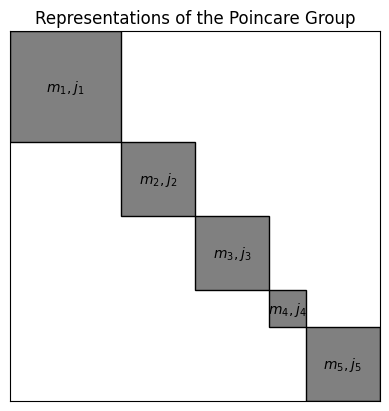
\includegraphics{irrep_visual.png}
\end{figure}

Here we have a direct sum of the irreducible representations of the Poincare group. Each irreducible representation is labelled by differnet values of $P^2$ and $W^2$, which we have labelled with the more physically recognizable mass and spin. 

So a Poincare transformation can only mix together states that form each irreducible representation. If we keep with the notion of mass and spin, this means that states will always get mixed with other states that have the same mass and spin. The momentum and spin projection will get mixed together, but we will never send a state with mass $m_1$ to a different state with mass $m_2$.

This is exactly what we expect out of a particle: a particle should have a definite mass and spin value. Lorentz transformations and translations should be able to chagne a particle's momentum and spin projection, but it will never change its mass or spin. Thus, we can associate each irreducible representation of the Poincare group as a different particle. Each block on the visual above represents a different particle, and Poincare transformations only mix together states from the same particle. 

Let's stop and think about why we just spent so long coming up with the definition of a particle. We could have said that particles are some sort of physical objects that carry with them mass and spin among other things and essentially define particles by what we observe. However, what we have done here is more fundamental - all we have stated is that particles transform like irreducible representaitons of the Poincare group. And by defining particles that way, we are automatically are given the property of mass and spin from Poincare invariance.


\section{Massive Particles}
\section{Massless Particles}

\section{Introduction}
The Poincare group is a combination of the translation group, which consists of translations in the 4 dimensions of spacetime, and the Lorentz group, which consists of boosts, rotations, parity, and time reversal. It is of particular interest to us because \aside{every relativistic theory we come up with must be Poincare invariant}{Ignoring general relativity, in which Poincare invariance is only local.}.


As we will see throughout these notes, we will define a particle to "be" irreducible representations of the Poincare group. Then simply requiring our theories to be Poincare invariant automatically means all our particles gain the fundamental properties of mass and spin. I find this notion particularly important - we could have defined particles to have mass and spin because that is what we observe experimentally. However, by being more abstract about what we think about particles, our only assumption is now that the universe is Poincare invariant, and we get these properties for free.

Perhaps I have gotten too far ahead of myself. By the end of these notes, we should understand everything that I have said above. Here is an outline for where we will be going:

\section{Poincare Group}
As was mentioned in the introduction, the Poincare group consists of spacetime translations, Lorentz boosts, and rotations. It also contains parity and time-reversal, though we will largely ignore these. There are 4 degrees of freedom for translations (1 time and 3 spatial), so we expect 4 generators. We can put these into a 4-vector and call the generators $P_\mu$. Boosts and rotations have 6 degrees of freedom (3 boost parameters and 3 rotation angles), so we expect 6 generators. We could call these $M_i$ for $i=1.\dots6$, though that doesn't really match with our standard physics notation. Instead, we will use two indices $M_{\mu\nu}$ and require that this is anti-symmetric: $M_{\mu\nu}=-M_{\nu\mu}$. Note that \textit{each} of these is an entire matrix. If we wanted to use index notation to specify a specific element, we would say $(M^{\mu\nu})_{\alpha\beta}$.

Note that all we have assumed here is the number of degrees of freedom for translations, boosts, and rotations. It may seem that I have assumed $P_\mu$ is momentum and $M_{\mu\nu}$ needs to be antisymmetric, but all I have done is use a notation that will make things easier in the future. We have the benefit of knowing where we want to go, so using the best notation is an advantage.

Like we mentioned before, we will identify irreducible representations of the Poincare group with the notion of particles. We aren't there yet to fully make this connection, but it gives you an idea of where we need to go. So, we should focus on finding the different irreps and classifying their basis states. The basis states will be labelled by the eigenvalues of the maximal set of commuting generators. So, we should try and find the commutation relations between the generators $P_{\mu}$ and $M_{\mu\nu}$ so that we can label the eigenstates.

\subsection{Finding Commutation Relations}
\subsubsection{Group Multiplation Law}
We start our journey by finding the group multiplication law for the Poincare group. We will use the notation $(\Lambda,a)$ to define an ordered pair of Lorentz transformation $\Lambda$ and translation $a$ that represents a Poincare transformation. The Poincare transformation acts on the coordinate $x^\mu$ as equation \ref{eqn:poincare_transform}.
\begin{equation}
    x^\mu \rightarrow {\Lambda^\mu}_\nu x^\nu + a^\mu
    \label{eqn:poincare_transform}
\end{equation}

Let's then act with a second Poincare transformation.
\begin{equation}
    x^\mu \rightarrow {(\Lambda_1)^\mu}_\nu x^\nu + a^\mu \rightarrow {(\Lambda_2)^\mu}_\nu({(\Lambda_1)^\nu}_\alpha x^\alpha + a_1^\nu) + a_2^\mu = {(\Lambda_2)^\mu}_\nu{(\Lambda_1)^\nu}_\alpha x^\alpha+{(\Lambda_2)^\mu}_\nu a_1^\nu + a_2^\mu
\end{equation}

Thus, we see that two Poincare transformations give us the multiplication law $(\Lambda_2\Lambda_1,\Lambda_2 a_1 + a_2)$.

This implies that the action of a translation and Lorentz transformation together can be split into two separate group elements. This notation just means that we multiple the two group elements together, or in other words apply the transformations successively.
\begin{equation}
    (\Lambda,a)=(\Lambda,0)(\mathbb{1},a)
\end{equation}

Note that this is not an Abelian group, so the opposite ordering does not work. In fact, we will use this opposite ordering later when finding the commutation relations.
\begin{equation}
    (\Lambda,a)\neq (\mathbb{1},a)(\Lambda,0)
\end{equation}

\subsubsection{Inverse Element}
Armed with the group multiplication law, we can find the inverse element for a group. The identity element is clearly $(\mathbb{1}, 0)$, so we need $\Lambda_2\Lambda_1=\mathbb{1}$ and $\Lambda_2a_1+a_2=0$. This gives us $\Lambda_2=\Lambda_1^{-1}$ and $a_2=-\Lambda_1^{-1}a_1$. Thus, our inverse element ordered pair is $(\Lambda^{-1},-\Lambda^{-1}a)$.

\subsubsection{Infinitesimal Transformation}
An infinitesimal Lorentz transformation can be expanded in a Taylor series as ${\Lambda^\mu}_\nu={\delta^\mu}_\nu+{\omega^\mu}_\nu+\cdots$. By definition of the Lorentz group, $\Lambda^Tg\Lambda=g$, or, in index notation,
\begin{equation}
    {(\Lambda^T)_\alpha}^\mu g_{\mu\nu} {(\Lambda)^\nu}_\beta={\Lambda^\mu}_\alpha g_{\mu\nu} {(\Lambda)^\nu}_\beta=g_{\alpha\beta}
\end{equation}

We can raise and lower some indices using the metric to get this in a more useful form. We use ${g^\mu}_\nu={\delta^\mu}_\nu$, where $\delta$ is the Kronecker delta.
\begin{equation}
    {\Lambda^\mu}_\alpha \Lambda_{\mu\beta}=g_{\alpha\beta}\rightarrow {\Lambda_\mu}^\alpha {\Lambda^\mu}_\beta={\delta^\alpha}_\beta
\end{equation} 

Now we can plug in our Taylor expansion and keep to first order.
\begin{align*}
    {\Lambda_\mu}^\alpha {\Lambda^\mu}_\beta&=({\delta_\mu}^\alpha+{\omega_\mu}^\alpha+\dots)({\delta^\mu}_\beta+{\omega^\mu}_\beta+\cdots) \\
    &= {\delta_\mu}^\alpha{\delta^\mu}_\beta+{\delta_\mu}^\alpha{\omega^\mu}_\beta+{\omega_\mu}^\alpha{\delta^\mu}_\beta+\dots\\
    &={\delta^\alpha}_\beta+{\omega^\alpha}_\beta+{\omega_\beta}^\alpha+\dots
\end{align*}

This is true for arbitrary $\omega$, so it must hold that all powers of $\omega$ on both sides of the equation must be zero. Remember that this is equal to ${\delta^\alpha}_\beta$, so the 0th order term matches. Thus, we have that ${\omega^\alpha}_\beta+{\omega_\beta}^\alpha=0$, or
\begin{equation}
    {\omega^\alpha}_\beta=-{\omega_\beta}^\alpha
\end{equation}

\subsubsection{Representations}
Using our notation for a group element as $(\Lambda,a)$, we will define the representation of that group element to be $D(\Lambda,a)$. Our representation by definition follows the group multiplication law.
\begin{equation}
    D(\Lambda_2,a_2)D(\Lambda_1,a_1)=D(\Lambda_2\Lambda_1,\Lambda_2a_1+a_2)
\end{equation}

And likewise our representations can be split into a representation of only translations and a representation of only Lorentz transformations.
\begin{equation}
    D(\Lambda,a)=D(\mathbb{1},a)D(\Lambda,0)
\end{equation}

Note that the order matters here, as
\begin{equation}
    D(\Lambda,0)D(\mathbb{1},a)=D(\Lambda,\Lambda a)
\end{equation}

We know that any group element can be found via an exponential of the generators, so we can write a representation for both translations and Lorentz transformations. The Lorentz transformations will be in terms of the parameter tensor $\alpha_{\mu\nu}$ that we just looked at.
\begin{align}
    D(\Lambda,0)&=e^{\frac{i}{2}\omega_{\mu\nu}M^{\mu\nu}} \\
    D(\mathbb{1},a)&=e^{ia_\mu P^\mu}
\end{align}

Becuase we defined $M^{\mu\nu}$ to be antisymmetric initially, $\alpha_{\mu\nu}M^{\mu\nu}$ is symmetric, so we divide by $2$ to avoid double counting $\alpha_{\mu\nu}M^{\mu\nu}$ and $\alpha_{\nu\mu}M^{\nu\mu}$. As we will see, this factor of $\frac{1}{2}$ will also come in handy later when finding the commutation relations.

\subsubsection{At Long Last}
We finally have all the tools necessary to find the commutation relations between the generators. Let's start with the translation generators $P^\mu$. We can combine two translations as $D(\mathbb{1},a_1)D(\mathbb{1},a_2)=D(\mathbb{1},a_1+a_2)$. Let's expand both sides of this equation.
\begin{align*}
    &\text{LHS: }(1+i (a_1)_\mu P^\mu-\frac{1}{2}(a_1)_\mu P^\mu (a_1)_\nu P^\nu +\dots)(1+i (a_2)_\mu P^\mu-\frac{1}{2}(a_2)_\mu P^\mu (a_2)_\nu P^\nu+\dots) \\
    &=1+i[(a_1)_\mu+(a_2)_\mu]P^\mu-\frac{1}{2}(a_1)_\mu P^\mu (a_1)_\nu P^\nu-\frac{1}{2}(a_2)_\mu P^\mu (a_2)_\nu P^\nu-(a_1)_\mu P^\mu (a_2)_\nu P^\nu+\dots
\end{align*}

Now we look at the right hand side.
\begin{align*}
    \text{RHS: }1&+i[(a_1)_\mu+(a_2)_\mu]P^\mu-\frac{1}{2}[(a_1)_\mu+(a_2)_\mu]P^\mu[(a_1)_\nu+(a_2)_\nu]P^\nu+\dots \\
    &=1+i[(a_1)_\mu+(a_2)_\mu]P^\mu-\frac{1}{2}(a_1)_\mu(a_1)_\nu P^\mu P^\nu -\frac{1}{2}(a_2)_\mu(a_2)_\nu P^\mu P^\nu \\
    &\qquad-\frac{1}{2}(a_1)_\mu(a_2)_\nu P^\mu P^\nu-\frac{1}{2}(a_2)_\mu(a_1)_\nu P^\mu P^\nu+\dots
\end{align*}

If we equate these two sides, several of the terms cancel. We will look specifically at 2nd order terms and omit writing any higher orders.
\begin{align*}
    -(a_1)_\mu P^\mu (a_2)_\nu P^\nu&=-\frac{1}{2}(a_1)_\mu(a_2)_\nu P^\mu P^\nu-\frac{1}{2}(a_2)_\mu(a_1)_\nu P^\mu P^\nu
\end{align*}

We now collect like terms.
\begin{align*}
    \frac{1}{2}(a_1)_\mu(a_2)_\nu P^\mu P^\nu-\frac{1}{2}(a_2)_\mu(a_1)_\nu P^\mu P^\nu = 0
\end{align*}

For the last step, we rename $\mu\rightarrow\nu$ and vice versa in the second term. This is so we can take out the $a_1$ and $a_2$ parameters from both terms.
\begin{align*}
    \frac{1}{2}(a_1)_\mu(a_2)_\nu P^\mu P^\nu-\frac{1}{2}(a_2)_\nu(a_1)_\mu P^\nu P^\mu &= 0 \\
    \frac{1}{2}(a_1)_\mu(a_2)_\nu [P^\mu,P^\nu]&=0
\end{align*}

This must hold true for arbitary $a_1$ and $a_2$, so we conclude that $[P^\mu,P^\nu]=0$.

To find the commutation relations between two translation generators, we looked at $D(\mathbb{1},a_1)D(\mathbb{1},a_2)$. So, to find the commutation relations between $M^{\mu\nu}$ and $P^\mu$, you may expect that we will look at $D(\Lambda,0)D(\mathbb{1},a)=D(\Lambda,\Lambda a)$. Remembering that we can split up a representation into a pure translation and pure Lorentz transformation, this becomes
\begin{equation}
    D(\Lambda,0)D(\mathbb{1},a)=D(\mathbb{1},\Lambda a)D(\Lambda, 0)
\end{equation}

Now we can expand both sides by Taylor expanding $e^{\frac{i}{2}\omega_{\mu\nu}M^{\mu\nu}}=1+\frac{i}{2}\omega_{\mu\nu}M^{\mu\nu}+\dots$.
\begin{align*}
    (1+\frac{i}{2}\omega_{\mu\nu}M^{\mu\nu}+\dots)(1+ia_\mu P^\mu+\dots)&=(1+i{\Lambda_\mu}^\nu a_\nu P^\mu +\dots)(1+\frac{i}{2}\omega_{\mu\nu}M^{\mu\nu}+\dots)
\end{align*}

Now we multiply both sides out. However, we should make sure to also expand ${\Lambda_\mu}^\nu a_\nu=({\delta_\mu}^\nu+{\omega_\mu}^\nu+\dots)a_\nu$. We will write everything up to second order.
\begin{align*}
    1+\frac{i}{2}\omega_{\mu\nu}M^{\mu\nu}+ia_\mu P^\mu&-\frac{1}{2}\omega_{\mu\nu}a_\sigma M^{\mu\nu}P^\sigma+\dots= \\
    &1+\frac{i}{2}\omega_{\mu\nu}M^{\mu\nu}+ia_\mu P^\mu+i{\omega_\mu}^\nu a_\nu P^\mu-\frac{1}{2}\omega_{\mu\nu}a_\sigma P^\sigma M^{\mu\nu}+\dots
\end{align*}

Many terms cancel, and we can rearrange the remaining terms to give us an expression for the commutators.
\begin{align*}
    -\frac{1}{2}\omega_{\mu\nu}a_\sigma[M^{\mu\nu},P^\sigma]&=i{\omega_\mu}^\nu a_\nu P^\mu \\
    &= i g^{\nu\sigma} \omega_{\mu\nu} a_\sigma P^\mu
\end{align*}

You may be tempted to cancel off the $\omega_{\mu\nu}$ and $a_\sigma$ right now, but we can't do that quite yet. This is because this equality holds for the \textit{sum} over indices (remember summation notation!). So while the sum is equal, that doesn't necessarily the terms we have written out are equal. Now, in an equation written like below, if all the variables are independent of each other, then term by term the coefficients must be equal.
\begin{align*}
    a_0 x_0 + a_1 x_1 + a_2 x_2 + \dots = b_0 x_0 + b_1 x_1 + b_2 x_2 + \dots \rightarrow a_0 = b_0\text{, }a_1 = b_1\text{, etc.}
\end{align*}

However, all the values of $\omega_{\mu\nu}$ in our expression about aren't independent because $\omega_{\mu\nu}=-\omega_{\nu\mu}$. Thus, we need to look at the terms for both $\omega_{\mu\nu}$ and $\omega_{\nu\mu}$ and set those equal to each other.
\begin{align*}
    -\frac{1}{2}\omega_{\mu\nu}a_\sigma[M^{\mu\nu},P^\sigma]-\frac{1}{2}\omega_{\nu\mu}a_\sigma[M^{\nu\mu},P^\sigma]=i g^{\nu\sigma} \omega_{\mu\nu} a_\sigma P^\mu+i g^{\mu\sigma} \omega_{\nu\mu} a_\sigma P^\nu
\end{align*}

Now we can use $\omega_{\mu\nu}=-\omega_{\nu\mu}$ and collect like terms.
\begin{align*}
    -\omega_{\mu\nu}a_\sigma[M^{\mu\nu},P^\sigma]=i \omega_{\mu\nu} a_\sigma(g^{\nu\sigma} P^\mu- g^{\mu\sigma} P^\nu)
\end{align*}

Now we are able to make the claim that this holds for arbitrary $\omega_{\mu\nu}$ and $a_\sigma$, so we can ignore them.
\begin{equation}
    [M^{\mu\nu},P^\sigma]=i(g^{\mu\sigma} P^\nu-g^{\nu\sigma} P^\mu)
\end{equation}

Why didn't we have to be this careful when finding $[P^\mu,P^\nu]$ you may ask. In that case, all values of $a_\mu$ were indeed independent. The only reason we needed to go through these extra steps, in which we symmetrized the right hand side, was because of the non-independence of $\omega_{\mu\nu}$. We will have to do this again for our final commutation relation as well.

Now we seek the last commutation relation, $[M^{\mu\nu},M^{\rho\sigma}]$. In the same spirit as the previous two, we will look at the composition of two pure Lorentz transformations $D(\Lambda_1,0)D(\Lambda_2,0)=D(\Lambda_1\Lambda_2)$. But we need to know what $D(\Lambda_1\Lambda_2)$ looks like.
\begin{align*}
    \Lambda_1\Lambda_2&=({\delta^\mu}_\alpha+{\omega_1^\mu}_\alpha+\dots)({\delta^\alpha}_\nu+{\omega_2^\alpha}_\nu+\dots) \\
    &={\delta^\mu}_\nu+{\omega_1^\mu}_\nu+{\omega_2^\mu}_\nu+{\omega_1^\mu}_\alpha{\omega_2^\alpha}_\nu+\dots
\end{align*}

We then have our representation of $D(\Lambda_1\Lambda_2)=\text{exp}(\frac{i}{2}[(\omega_1)_{\mu\nu}+(\omega_2)_{\mu\nu}+(\omega_1)_{\mu\alpha}{(\omega_1)^\alpha}_\nu]M^{\mu\nu})$. \textbf{Why do I need to include up to 2nd order? I understand that I am looking at second order, so it makes sense that I would need to keep it. But the definition of the exponential should just be first order?}

Now we plug everything in. Let's first look at the left-hand side because the equation will be too long otherwise.
\begin{align*}
    (1+\frac{i}{2}(\omega_1)_{\mu\nu}M^{\mu\nu}&-\frac{1}{8}(\omega_1)_{\mu\nu}(\omega_1)_{\rho\sigma}M^{\mu\nu}M^{\rho\sigma}+\dots)(1+\frac{i}{2}(\omega_2)_{\mu\nu}M^{\mu\nu}-\frac{1}{8}(\omega_2)_{\mu\nu}(\omega_2)_{\rho\sigma}M^{\mu\nu}M^{\rho\sigma}+\dots) \\
    &=1+\frac{i}{2}[(\omega_1)_{\mu\nu}+(\omega_2)_{\mu\nu}]M^{\mu\nu}-\frac{1}{8}[(\omega_1)_{\mu\nu}(\omega_1)_{\rho\sigma}+(\omega_2)_{\mu\nu}(\omega_2)_{\rho\sigma}]M^{\mu\nu}M^{\rho\sigma} \\
    &-\frac{1}{4}(\omega_1)_{\mu\nu}(\omega_2)_{\rho\sigma}M^{\mu\nu}M^{\rho\sigma}+\dots
\end{align*}

Now we can look at the right-hand side.
\begin{align*}
    1&+\frac{i}{2}[(\omega_1)_{\mu\nu}+(\omega_2)_{\mu\nu}+(\omega_1)_{\mu\alpha}{(\omega_2)^\alpha}_\nu]M^{\mu\nu} \\
    &-\frac{1}{8}[(\omega_1)_{\mu\nu}+(\omega_2)_{\mu\nu}+(\omega_1)_{\mu\alpha}{(\omega_2)^\alpha}_\nu][(\omega_1)_{\rho\sigma}+(\omega_2)_{\rho\sigma}+(\omega_1)_{\rho\alpha}{(\omega_2)^\alpha}_\sigma]M^{\mu\nu}M^{\rho\sigma}+\dots
\end{align*}

After cancelling matching terms, we are left with the following to 2nd order.
\begin{align*}
    -\frac{1}{4}(\omega_1)_{\mu\nu}(\omega_2)_{\rho\sigma}M^{\mu\nu}M^{\rho\sigma}=\frac{i}{2}(\omega_1)_{\mu\alpha}{(\omega_2)^\alpha}_\nu M^{\mu\nu}-\frac{1}{8}(\omega_1)_{\mu\nu}(\omega_2)_{\rho\sigma}M^{\mu\nu}M^{\rho\sigma}-\frac{1}{8}(\omega_2)_{\mu\nu}(\omega_1)_{\rho\sigma}M^{\mu\nu}M^{\rho\sigma}
\end{align*}

We can rearrange now and shuffle indices in the last term to get the commutator.
\begin{align*}
    -\frac{1}{8}(\omega_1)_{\mu\nu}(\omega_2)_{\rho\sigma}[M^{\mu\nu},M^{\rho\sigma}]&=\frac{i}{2}(\omega_1)_{\mu\alpha}{(\omega_2)^\alpha}_\nu M^{\mu\nu} \\
    &= \frac{i}{2}(\omega_1)_{\mu\nu}(\omega_2)_{\rho\sigma} g^{\rho \nu}M^{\mu\sigma}
\end{align*}

We must go through the same procedure as before where we need to consider both $\omega_{\mu\nu}$ and $\omega_{\nu\mu}$. As the left hand side is symmetric under this switch (and the $\rho\leftrightarrow\sigma$ switch), we simply get 4 times what we already have.
\begin{align*}
    -\frac{1}{2}(\omega_1)_{\mu\nu}(\omega_2)_{\rho\sigma}[M^{\mu\nu},M^{\rho\sigma}]&=\frac{i}{2}(\omega_1)_{\mu\nu}(\omega_2)_{\rho\sigma}(g^{\rho \nu}M^{\mu\sigma}-g^{\rho \mu}M^{\nu\sigma}-g^{\sigma \nu}M^{\mu\rho}+g^{\sigma \mu}M^{\nu\rho})
\end{align*}

Thus, we have our commutation relations.
\begin{equation}
    [M^{\mu\nu},M^{\rho\sigma}]=i(g^{\rho \mu}M^{\nu\sigma}+g^{\sigma \nu}M^{\mu\rho}-g^{\sigma \mu}M^{\nu\rho}-g^{\rho \nu}M^{\mu\sigma})
\end{equation}

\end{document}
